\documentclass{beamer}

\usepackage{array}
\usepackage{dsfont}
\usepackage[normalem]{ulem}

\makeatletter
\def\input@path{{../figures/}}
\makeatother
\graphicspath{{../figures/}}

\newcommand{\tinyspace}{\mspace{1mu}}
\newcommand{\comment}[1]{\textcolor{blue}{%
  \begin{quote}\sf [*** #1 ***]\end{quote}}}

\def\I{\mathds{1}}

\newcommand{\abs}[1]{\lvert #1 \rvert}
\newcommand{\bigabs}[1]{\bigl\lvert #1 \bigr\rvert}
\newcommand{\Bigabs}[1]{\Bigl\lvert #1 \Bigr\rvert}
\newcommand{\biggabs}[1]{\biggl\lvert #1 \biggr\rvert}
\newcommand{\Biggabs}[1]{\Biggl\lvert #1 \Biggr\rvert}

\newcommand{\ip}[2]{\langle #1 , #2\rangle}

\newcommand{\bigip}[2]{\bigl\langle #1, #2 \bigr\rangle}
\newcommand{\Bigip}[2]{\Bigl\langle #1, #2 \Bigr\rangle}
\newcommand{\biggip}[2]{\biggl\langle #1, #2 \biggr\rangle}
\newcommand{\Biggip}[2]{\Biggl\langle #1, #2 \Biggr\rangle}

\newcommand{\norm}[1]{\lVert\tinyspace #1 \tinyspace\rVert}
\newcommand{\bignorm}[1]{\bigl\lVert\tinyspace #1 \tinyspace\bigr\rVert}
\newcommand{\Bignorm}[1]{\Bigl\lVert\tinyspace #1 \tinyspace\Bigr\rVert}
\newcommand{\biggnorm}[1]{\biggl\lVert\tinyspace #1 \tinyspace\biggr\rVert}
\newcommand{\Biggnorm}[1]{\Biggl\lVert\tinyspace #1 \tinyspace\Biggr\rVert}

\newcommand{\tr}{\operatorname{Tr}}
\newcommand{\class}[1]{\mathsf{#1}}

\renewcommand{\thefootnote}{\footnotesize{$\mathparagraph$}} 

\def\X{\mathcal{X}}
\def\Y{\mathcal{Y}}
\def\E{\mathcal{E}}
\def\K{\mathcal{K}}
\def\W{\mathcal{W}}
\def\C{\mathcal{C}}
\def\A{\mathcal{A}}
\def\B{\mathcal{B}}
\def\H{\mathcal{H}}
\def\R{\mathcal{R}}
\def\S{\mathcal{S}}
\def\complex{\mathbb{C}}
\def\real{\mathbb{R}}

\def\Q{\mathcal{Q}}
\def\L{\mathcal{L}}
\def\NS{\mathcal{NS}}

\def\BB84{\mathsf{BB84}}
\def\CHSH{\mathsf{CHSH}}

\def \GammaA{\Gamma_{\reg{A}}}
\def \GammaB{\Gamma_{\reg{B}}}
\def \SigmaA{\Sigma_{\reg{A}}}
\def \SigmaB{\Sigma_{\reg{B}}}

\def\ns{\textnormal{ns}}

\newcommand{\setft}[1]{\mathrm{#1}}
\newcommand{\Density}{\setft{D}}
\newcommand{\Pos}{\setft{Pos}}
\newcommand{\Proj}{\setft{Proj}}
\newcommand{\Unitary}{\setft{U}}
\newcommand{\Herm}{\setft{Herm}}
\newcommand{\Lin}{\setft{L}}
\newcommand{\Sep}{\setft{Sep}}
\newcommand{\LOCC}{\setft{LOCC}}
\newcommand{\Ent}{\setft{Ent}}

\def \im{\textnormal{im}}

\newcommand{\microspace}{\mspace{0.5mu}}
\newcommand{\ket}[1]{
  \lvert\microspace #1 \microspace \rangle}
\newcommand{\bra}[1]{
  \langle\microspace #1 \microspace \rvert}

\def\eps{\varepsilon}
\newcommand{\mh}{\textnormal{-}}

\newcommand{\reg}[1]{\mathsf{#1}}

\usepackage{colortbl}
\definecolor{Gray}{gray}{0.90}

\newtheorem{prop}[theorem]{Proposition}

\AtBeginSection[]{
  \begin{frame}
  \vfill
  \centering
  \begin{beamercolorbox}[sep=8pt,center,shadow=true,rounded=true]{title}
    \usebeamerfont{title}\insertsectionhead\par%
  \end{beamercolorbox}
  \vfill
  \end{frame}
}

\title{Bounding the Value of Extended Nonlocal Games}
\subtitle{Theory Seminar}
\author[V. Russo]{Vincent Russo}
\institute[UWaterloo]{University of Waterloo}
\date{September 15, 2016}
\titlegraphic{
\includegraphics[scale=0.5]{UW_IQC}}

\begin{document}
  {%
    \setbeamertemplate{headline}{}
    \frame{\titlepage}
  }

  \beamertemplatenavigationsymbolsempty
  \addtobeamertemplate{navigation symbols}{}{%
    \usebeamerfont{footline}%
    \usebeamercolor[fg]{footline}%
    \hspace{1em}%
    \insertframenumber/\inserttotalframenumber
  }
  \setbeamercolor{footline}{fg=black}
  % \setbeamerfont{footline}{series=\bfseries}

  \begin{frame}
    \frametitle{Outline}
    \tableofcontents%[part=1,pausesections]
  \end{frame}

%%%%%%%%%%%%%%%%%%%%%%%%%%%%%%%%%%%%%%%%%%%%%%%%%%%%%
  \section{Nonlocal games}
%%%%%%%%%%%%%%%%%%%%%%%%%%%%%%%%%%%%%%%%%%%%%%%%%%%%%

% Nonlocal games:
\begin{frame}
	\frametitle{Nonlocal games}
	A \emph{nonlocal game} is a cooperative game played between \emph{Alice} and \emph{Bob} against a \emph{referee}. 
	\begin{figure}[!htpb] \label{fig:nonlocal-game}
	\begin{center}
		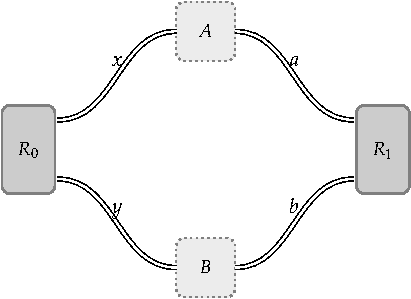
\includegraphics[scale=0.8]{figures/two_player_game.pdf}
	\end{center}
\end{figure}
	\begin{enumerate}
		\item Question and answer sets: $(\SigmaA, \SigmaB)$ and $(\GammaA, \GammaB)$,
		\item Distributions on question pairs: $\pi: \SigmaA \times \SigmaB \rightarrow [0,1]$ ,
		\item A predicate $V : \GammaA \times \GammaB \times \SigmaA \times \SigmaB \rightarrow \{0,1\}$, where 
\[
 V(a,b|x,y) =
  \begin{cases} 
      \hfill 1 \hfill & \text{ if Alice and Bob \textcolor{green}{win}}, \\
      \hfill 0 \hfill & \text{ if Alice and Bob \textcolor{red}{lose}}. \\
  \end{cases}
\]			
	\end{enumerate}
\end{frame}

\begin{frame}
	\frametitle{Strategies for nonlocal games}
	Alice and Bob could use different types of \emph{strategies}:
	\vspace{2mm}
	\begin{itemize}
		\item \emph{Classical strategies:} Alice and Bob answer deterministically, determined by functions of $f : \SigmaA \rightarrow \GammaA$ and $g : \SigmaB \rightarrow \GammaB$.
		\vspace{5mm}
		\item \emph{Quantum strategies:} Alice and Bob share a joint quantum system $\rho \in \Density(\A \otimes \B)$ and allow their answers to be outcomes of measurements on this shared system.		
		\vspace{5mm}
		\item \emph{Commuting measurement strategies:} Alice and Bob share a quantum system over a single Hilbert space $\rho \in \Density(\H)$ and allow their answers to be outcomes of measurements on this system. 
%		\vspace{5mm}
%		\item \emph{Non-signaling strategies:} No instantaneous communication between parties.  
	\end{itemize}
\end{frame}

\begin{frame}
	\frametitle{Winning probabilities for Alice and Bob}
	For any type of strategy, the output probability distribution produced by Alice and Bob may be described by a \emph{correlation operator}:
	\begin{align*}
		C \in \Lin(\real^{\SigmaA \times \GammaA}, \real^{\SigmaB \times \GammaB}),
	\end{align*}
where $C((x,a),(y,b))$ is the probability that Alice and Bob output $(a,b)$ given questions $(x,y)$. 
\pause
\vspace{5mm}

For a nonlocal game, the probability that Alice and Bob win for a given choice of $x,y,a,b$ is 
\begin{align*}
	\sum_{x,y} \pi(x,y) \sum_{a,b} V(a,b|x,y) C((x,a), (y,b)).
\end{align*}
\end{frame}

\begin{frame}
	\frametitle{Values for nonlocal games}
	The \emph{value} of a nonlocal game is the maximal winning probability for the players to win over all strategies of a specified type. 
	\vspace{2mm}
	
For a nonlocal game, $G$, we denote the classical and quantum values as 
	\begin{itemize}
		\item Classical value: $\omega(G)$,
		\item Commuting measurement value: $\omega_c(G)$,
		\item Quantum value: $\omega^*(G)$.
	\end{itemize}	
	\vspace{2mm}
	
	The values obey the following relationship for any nonlocal game:
	\begin{align*}
		\omega(G) \leq \omega^*(G) \leq \omega_c(G).
	\end{align*}
\end{frame}

\begin{frame}
	\frametitle{Quantum strategies for nonlocal games}
	A \emph{quantum strategy} consists of finite-dimensional complex Euclidean spaces $\A$ and $\B$ as well as the following:
	\begin{itemize}
		\item Shared state: $\rho \in \A \otimes \B$.
		\item Measurements $\{A^x_a\} \subset \Pos(\A)$ and $\{B_b^y\} \subset \Pos(\B)$.
	\end{itemize}
	\pause 
	\vspace{5mm}
	Winning probability for a quantum strategy is given by:
	\begin{align*}
		\sum_{x,y} \pi(x,y) \sum_{a,b} V(a,b|x,y) \bigip{A_a^x \otimes B_b^y}{\rho}.
	\end{align*}
	The \emph{quantum value}, denoted as as $\omega^*(G)$, is the supremum of the winning probability over all quantum strategies. 
\end{frame}

\begin{frame}
	\frametitle{Commuting measurement strategies for nonlocal games}
	A \emph{commuting measurement strategy} consists of a single (possibly infinite-dimensional) complex Euclidean space $\H$, as well as the following:
	\begin{itemize}
		\item Shared state: $\rho \in \H$.
		\item Measurements $\{A^x_a\} \subset \Pos(\H)$ and $\{B_b^y\} \subset \Pos(\H)$,
	\end{itemize}
	such that $\left[A_a^x, B_b^y\right] = 0$ for all $x,y,a,b$. 
	\vspace{5mm}
	
	Winning probability for a commuting measurement strategy is given by:
	\begin{align*}
		\sum_{x,y} \pi(x,y) \sum_{a,b} V(a,b|x,y) \bigip{A_a^x B_b^y}{\rho}.
	\end{align*}
	The \emph{commuting measurement value}, denoted as as $\omega_c(G)$, is the supremum of the winning probability over all commuting measurement strategies. 
\end{frame}

\begin{frame}
	\frametitle{Optimizing over quantum strategies is hard}
	\begin{center}
		{Want: Method to calculate the quantum value of a nonlocal game.}
	\end{center}	
	\vspace{2mm}
	This figure shows representations of the space of correlations for fixed and finite number of possible questions and answers.
	\begin{figure}[!htpb] \label{fig:extended-nonlocal-game}
	\begin{center}
		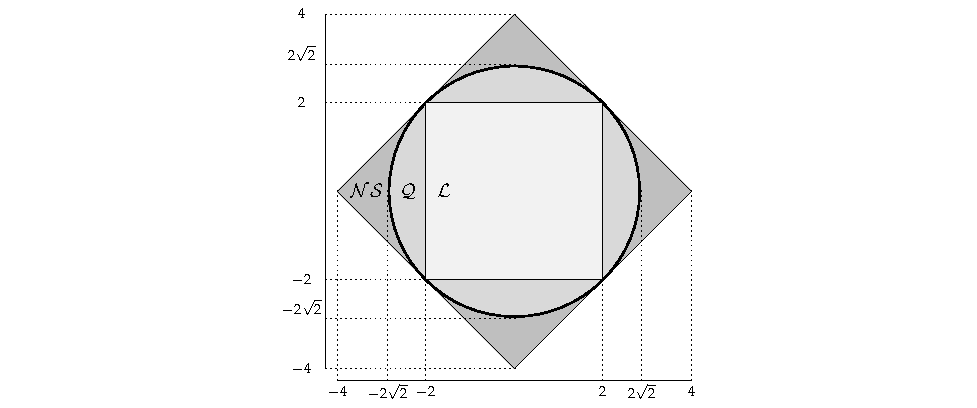
\includegraphics[scale=0.65]{figures/chsh_polytope.pdf}
	\end{center}
\end{figure}	
	Unfortunately, the set $\Q$ is a non-polyhedral set with an infinite number of extreme points. 
\end{frame}

%%%%%%%%%%%%%%%%%%%%%%%%%%%%%%%%%%%%%%%%%%%%%%%%%%%%%
  \section{Upper bounding nonlocal games}
%%%%%%%%%%%%%%%%%%%%%%%%%%%%%%%%%%%%%%%%%%%%%%%%%%%%%

\begin{frame}
	\frametitle{Upper bounds for nonlocal games}
	\begin{itemize}
		\item The NPA hierarchy\footnote{[Navascu\'es, Pironio, and Ac\'in, (2008)]} is a method of placing \emph{upper bounds} on the \emph{quantum value} of nonlocal games. 
		\item Hierarchy of semidefinite programs is \emph{guaranteed} to converge to the commuting measurement value for some finite level, $\ell$ of the hierarchy. 
		\item The commuting measurement value is an upper bound on the quantum value, $\omega^*(G) \leq \omega_c(G)$, for all nonlocal games, $G$. 
	\end{itemize}
	\begin{center}
		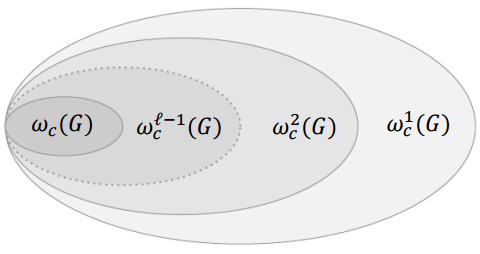
\includegraphics[scale=0.5]{figures/CommutingValues}
	\end{center}
\end{frame}

%\begin{frame}
%	\frametitle{Commuting measurement strategies}
%A \emph{commuting measurement strategy} consists of a \emph{state} and \emph{measurements}
%	\begin{itemize}
%		\item State: $\rho \in \Density(\H)$,
%		\item Measurements: $\{A_a^x\}$, $\{B_b^y\}$\footnote{where $\left[A_a^x, B_b^y\right] = 0$ for all $\{A_a^x\}, \{B_b^y\} \in \Pos(\H)$.}
%	\end{itemize}
%	\vspace{5mm}
%
%	The winning probability for a given choice of $x,y,a,b$ is:
%	\begin{align*}
%		\sum_{x,y} \pi(x,y) \sum_{a,b} V(a,b|x,y) \ip{A_a^x B_b^y}{\rho}
%	\end{align*}
%		The \emph{commuting measurement value} of a nonlocal game, $\omega_c(G)$, is the supremum of the winning probability over all commuting measurement strategies
%\end{frame} 

\begin{frame}
	\frametitle{NPA theorem (Main idea)}
	\begin{itemize}
		\item Finding a quantum state and measurements for a quantum strategy is a computationally difficult task. 
		\pause
		\item Instead then, let's think about a set of \emph{weaker} conditions that correspond to a commuting measurement strategy. 
		\pause
		\item In the NPA hierarchy, each condition amounts to verifying the existence of a positive semidefinite matrix with structure that depends on algebraic properties satisfied by a commuting measurement strategy. 
		\pause
		\item If any of these conditions are violated, we may conclude that there does not exist an adequate state and sets of measurements. 
	\end{itemize}
\end{frame}   

\begin{frame}
	\frametitle{NPA theorem (Main idea)}
	NPA states that there exists some matrix \textcolor{blue}{$C^{(\ell)}$} that allows $\omega_c(G)$ to be calculated by maximizing
	\begin{align*}
		\sum_{x,y,a,b} \pi(x,y) V(a,b|x,y) \textcolor{blue}{C^{(\ell)}((x,a),(y,b))}
	\end{align*}
	for some finite level, $\ell$, such that \textcolor{blue}{$C^{(\ell)}$} satisfies certain linear constraints. 
	\vspace{5mm}
	
	\begin{itemize}
		\item These linear constraints can be checked via SDP! 
		\item The next few slides will describe how \textcolor{blue}{$C^{(\ell)}$} is defined.
	\end{itemize}
	
\end{frame}

\begin{frame}
	\frametitle{PSD operator}
	\comment{More on intuition behind the $C^{(\ell)}$ operator.}
\end{frame}

\begin{frame}
	\frametitle{Strings}
	In order to index into $C^{(\ell)}((x,a),(y,b))$, we will consider strings. 
	\vspace{5mm}
		
	Define alphabets 
	\begin{align*}
		\SigmaA = X \times A, \quad \SigmaB = Y \times B, \quad \Sigma^* = \{\epsilon\} \cup \SigmaA \cup \SigmaB. 
	\end{align*}

For example, we can refer to operators (or products of operators) as tuples of concatenated strings. For example:
\begin{equation}
	\begin{aligned}
		&A_a^x \rightarrow (x,a), \quad \textnormal{and} \nonumber \\
		&A_{a_1}^{x_1} \cdots A_{a_k}^{x_k} \rightarrow (x_1,a_1) \cdots (x_k,a_k). \nonumber
	\end{aligned}
\end{equation}
Similarly for Bob.

\end{frame}

\begin{frame}
	\frametitle{Equivalence relations for strings}
The measurements in a commuting measurement strategy are \emph{projective} and they \emph{commute}. This property can be conveyed in terms of a string relation:
	\vspace{5mm}
	
	For all strings $s,t \in \Sigma^*$, 
	\begin{enumerate}
		\item Projective: $s \sigma t \sim s \sigma \sigma t$ for all $\sigma \in \Sigma$
		\item Commute: $s \sigma \tau t \sim s \tau \sigma t$ for all $\sigma \in \SigmaA$ and $\tau \in \SigmaB$. 
	\end{enumerate}
\end{frame}

\begin{frame}
	\frametitle{Admissible functions}	
	The function
		\begin{align*}
			\phi : \Sigma^* \rightarrow \complex
		\end{align*}
		is \emph{admissible} iff it satisfies the following conditions:
		\begin{enumerate}
			\item Measurements sum to identity:
				\begin{align*}
					\sum_a \phi(s(x,a)t) = \sum_b \phi(s(y,b)t) = \phi(st),
				\end{align*}
				for all $x,y \in X \times Y$. 
			\item Something:
				\begin{align*}
					\phi(s(x,a)(x,a^{\prime})t) = \phi(s(y,b)(y,b^{\prime})t) = 0
				\end{align*}
			\item For all $s,t \in \Sigma^*$ where $s \sim t$
				\begin{align*}
					\phi(s) = \phi(t).
				\end{align*}
		\end{enumerate}
\end{frame}

\begin{frame}
	\frametitle{$\ell$-th order admissible matrices}
	We call the matrix $C^{(\ell)}$ an \emph{$\ell$-th order admissible matrix} if 
	\begin{enumerate}
		\item There exists an admissible function 
			\begin{align*}
				\phi : \Sigma^{\leq 2 \ell} \rightarrow \complex,
			\end{align*}
			such that 
			\begin{align*}
				C^{(\ell)}(s,t) = \phi(s^{\tiny{R}}t) \quad \forall s,t \in \Sigma^{\leq \ell},
			\end{align*}
		\item Normalization: $C^{(\ell)}(\epsilon,\epsilon) = 1$,
		\item $C^{(\ell)}$ is positive semidefinite. 
	\end{enumerate}
\end{frame}

\begin{frame}
	\frametitle{$\ell$-th order pseudo commuting measurement assemblages}
	Define an \emph{$\ell$-th order pseudo commuting measurement assemblage} 
	\begin{align*}
		K: A \times B \times X \times Y \rightarrow \Lin(\complex),
	\end{align*}
	for which there exists an $\ell$-th order admissible matrix $C^{(\ell)}$ such that 
	\begin{align*}
		K(a,b|x,y) = C^{(\ell)}((x,a),(y,b)) \quad \forall x,y,a,b. 
	\end{align*}
\end{frame}

\begin{frame}
	\frametitle{Example}
	Consider a nonlocal game where $\abs{X} = \abs{Y} = \abs{A} = \abs{B} = 2$. Let's compute $C^{(1)}$:
	\[
\begin{aligned}
C^{(1)} =
\left(
\begin{array}{c||cccc|ccc}
 & \I & A_0^0 & \cdots & A_1^1 & B_0^0 & \cdots & B_1^1 \\
\hline\hline 
\I & & & & & & & \\
A_0^0 & & & & & & &  \\
\vdots & & & & & & & \\
A_1^1 & & & & & & & \\
\hline 
B_0^0 & & & & & & & \\
\vdots & & & & & & & \\
B_1^1 & & & & & & & 
\end{array}
\right) 
\end{aligned}
\]

\begin{itemize}
	\item Fill in matrix with products of row and column to generate element $Z$. 
	\item For each $Z$ computed in this way, the entry refers to an inner product between $Z$ and the shared state $\rho$, i.e. $\ip{Z}{\rho}$. 
\end{itemize}

\end{frame}

\begin{frame}
	\frametitle{Example}
	Consider a nonlocal game where $\abs{X} = \abs{Y} = \abs{A} = \abs{B} = 2$. Let's compute $C^{(1)}$:
	\[
\begin{aligned}
C^{(1)} =
\left(
\begin{array}{c||cccc|ccc}
 & \I & A_0^0 & \cdots & A_1^1 & B_0^0 & \cdots & B_1^1 \\
\hline\hline 
\I & \I & A_0^0 & \cdots & A_1^1 & B_0^0 & \cdots & B_1^1 \\
A_0^0 & A_0^0 & A_0^0 & \cdots & A_0^0 A_1^1 & A_0^0 B_0^0 & \cdots & A_0^0 B_1^1 \\
\vdots & \vdots & \vdots & \ddots & \vdots & \vdots  & \ddots & \vdots \\
A_1^1 & A_1^1 & A_1^1 A_0^0 & \cdots & A_1^1 & A_1^0 B_0^0 & \cdots & A_1^1 B_1^1 \\
\hline 
B_0^0 & B_0^0 & B_0^0 A_0^0 & \cdots & B_0^0 A_1^1 & B_0^0 & \cdots & B_0^0 B_1^1 \\
\vdots & \vdots & \vdots & \ddots & \vdots & \vdots  & \ddots & \vdots \\
B_1^1 & B_1^1 & B_1^1 A_0^0 & \cdots & B_1^1 A_1^1 & B_1^1 B_0^0 & \cdots & B_1^1
\end{array}
\right) 
\end{aligned}
\]
\end{frame}


%%%%%%%%%%%%%%%%%%%%%%%%%%%%%%%%%%%%%%%%%%%%%%%%%%%%%
  \section{Extended nonlocal games}
%%%%%%%%%%%%%%%%%%%%%%%%%%%%%%%%%%%%%%%%%%%%%%%%%%%%%    


% Extended nonlocal games:
\begin{frame}
	\frametitle{Extended nonlocal games}
	An \emph{extended nonlocal game} is a nonlocal game where the \emph{referee also holds a quantum system} that he measures provided by Alice and Bob. 
	\begin{figure}[!htpb] \label{fig:extended-nonlocal-game}
	\begin{center}
		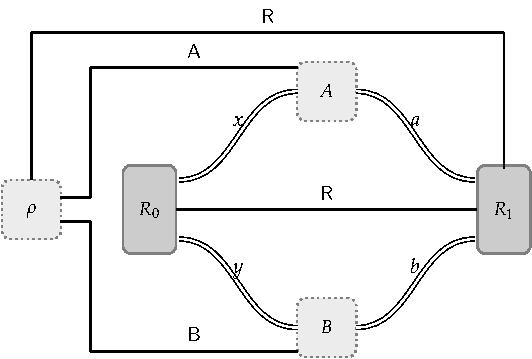
\includegraphics[scale=0.7]{figures/enlg_2.pdf}
	\end{center}
\end{figure}
	\begin{enumerate}
		\item Question and answer sets $(\SigmaA,\SigmaB)$ and $(\GammaA,\GammaB)$. \vspace{1mm}		
		\item Distribution on question pairs: $\pi: \SigmaA \times \SigmaB \rightarrow [0,1]$.\vspace{1mm}
		\item A measurement operator $V: \GammaA \times \GammaB \times \SigmaA \times \SigmaB \rightarrow \Pos(\R)$.
	\end{enumerate}
\end{frame}

\begin{frame}
	\frametitle{Extended nonlocal games: Winning and losing probabilities}
	At the end of the protocol, the referee has: 
		\begin{enumerate}
			\item The state at the end of the protocol: 
				\begin{align*}
					\rho_{a,b}^{x,y} \in \Density(\R).
				\end{align*}
			\item A measurement the referee makes on its part of the state $\rho$: 
			\begin{align*}
				V(a,b|x,y) \in \Pos(\R).
			\end{align*}				
		\end{enumerate}
	The respective winning and losing probabilities are given by
		\begin{align*}
			\biggip{V(a,b|x,y)}{\rho_{a,b}^{x,y}} \quad \textnormal{and} \quad \biggip{\I - V(a,b|x,y)}{\rho_{a,b}^{x,y}}. 
		\end{align*}
\end{frame}

% Intepreting the equation. The idea is that Alice and Bob perform their measurements, they're obtaining outcomes, and conditioned on those outcomes the referee is doing something and getting some result. 
\begin{frame}
	\frametitle{Standard quantum strategies}
	A \emph{standard quantum strategy} consists of finite-dimensional complex Euclidean spaces $\R,\A$, and $\B$ as well as the following:
	\begin{itemize}
		\item Shared state: $\rho \in \R \otimes \A \otimes \B$.

		\item Measurements: $\{ A_a^x \} \subset \Pos(\A), \quad \{ B_b^y \} \subset \Pos(\B)$.
	\end{itemize}
	\pause
	\vspace{5mm}
	Winning probability for a standard quantum strategy is given by:
	\begin{align*}
		\sum_{x,y} \pi(x,y) \sum_{a,b} \biggip{V(a,b|x,y) \otimes A_a^x \otimes B_b^y}{\rho}
	\end{align*}
	The \emph{standard quantum value}, denoted as $\omega^*(G)$, is the supremum of the winning probability over all standard quantum strategies.
\end{frame}

%%%%%%%%%%%%%%%%%%%%%%%%%%%%%%%%%%%%%%%%%%%%%%%%%%%%%
  \section{Upper bounding extended nonlocal games}
%%%%%%%%%%%%%%%%%%%%%%%%%%%%%%%%%%%%%%%%%%%%%%%%%%%%%


\begin{frame}
	\frametitle{Upper bounds for extended nonlocal games}
	\emph{Extended NPA hierarchy:}
	\begin{itemize}
		\item Uses the same idea as the NPA hierarchy. (For $\dim(\R) = 1$, the NPA hierarchy is a special case.)
		\item Enables one to compute \emph{upper bounds} on the \emph{standard quantum value} for \emph{extended nonlocal games}. 
		\item Same idea as before, only now we need to take into account the actions of the referee. 
	\end{itemize}
	\begin{center}
		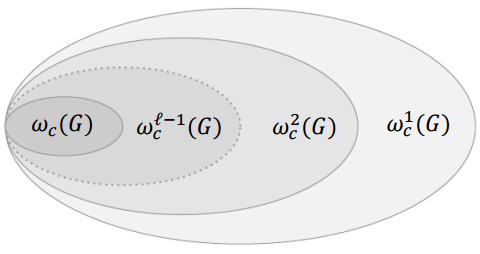
\includegraphics[scale=0.5]{figures/CommutingValues}
	\end{center}	
\end{frame}

\begin{frame}
	\frametitle{Commuting measurement strategies (for ENLG)}
	A \emph{commuting measurement strategy} consists of a finite-dimensional complex Euclidean space $\H$ as well as the following:
	\begin{itemize}
		\item Shared state: $\rho \in \R \otimes \H$.
		\item Measurements: $\{ A_a^x \} \subset \Pos(\H), \quad \{ B_b^y \} \subset \Pos(\H)$,
			
			where $[A_a^x, B_b^y] = 0$ for all $x,y,a,b$. 
	\end{itemize}
	\pause
	\vspace{5mm}
	The expected \emph{pay-off} for a commuting measurement strategy is given by:
	\begin{align*}
		\sum_{(x,y) \in \SigmaA \times \SigmaB} \pi(x,y) \sum_{(a,b) \in \GammaA \times \GammaB} \biggip{V(a,b|x,y) \otimes A_a^x B_b^y}{\rho}
	\end{align*}
	The \emph{commuting measurement value}, denoted as $\omega_c(G)$, is the supremum of the pay-off over all commuting measurement strategies.
\end{frame}

\begin{frame}
	\frametitle{Extended NPA theorem}
	There exists some matrix \textcolor{blue}{$M^{(\ell)}$} that allows $\omega_c(G)$ (where $G$ is an ENLG) to be calculated by maximizing 
	\begin{align*}
		\sum_{x,y,a,b} \pi(x,y) \biggip{V(a,b|x,y)}{\textcolor{blue}{M^{(\ell)}((x,a),(y,b))}}
	\end{align*}
\end{frame}

\begin{frame}
	\frametitle{Extended NPA hierarchy}
	Same idea, but now we're taking into account the referee, and therefore have a larger matrix.
		
	For each $\ell$, now consider block matrices
	\begin{align*}
		M^{(\ell)} = \begin{pmatrix} M_{1,1}^{(\ell)} & \cdots & M_{1,m}^{(\ell)} \\ \vdots & \ddots & \vdots \\ M_{m,1}^{(\ell)} & \cdots & M_{m,m}^{(\ell)} \end{pmatrix}
	\end{align*}
	where each block takes the form $M_{i,j}^{(\ell)} : \Sigma^{\leq \ell} \times \Sigma^{\leq \ell} \rightarrow \complex$. 
	\begin{itemize}
		\item Each submatrix has similar properties to what we saw for the NPA hierarchy. 
		\item The overall matrix also has some structure, which is unique to this case.
	\end{itemize}
\end{frame}


%%%%%%%%%%%%%%%%%%%%%%%%%%%%%%%%%%%%%%%%%%%%%%%%%%%%%
  \section*{Supplementary material}
%%%%%%%%%%%%%%%%%%%%%%%%%%%%%%%%%%%%%%%%%%%%%%%%%%%%%

%%%%%%%%%%%%%%%%%%%%%%%
% ENLG GAMES
%%%%%%%%%%%%%%%%%%%%%%%
  \begin{frame}[noframenumbering]
  \vfill
  \centering
  \begin{beamercolorbox}[sep=8pt,center,shadow=true,rounded=true]{title}
    \usebeamerfont{title}Supplementary material: \\ Extended nonlocal games
  \end{beamercolorbox}
  \vfill
  \end{frame}

\begin{frame}[noframenumbering]
	\frametitle{Winning probability for standard quantum strategies}
	The winning probability is given by the following equation:
	\small{
	\begin{align*}
		\sum_{x,y} \pi(x,y) \sum_{a,b} \frac{ \ip{V(a,b|x,y)}{\tr_{\A\otimes\B}\left(\I_{\R} \otimes A_a^x \otimes B_b^y)\rho\right)} }{\tr(\I_{\R} \otimes A_a^x \otimes B_b^y) \rho)} \tr(\I_{\R} \otimes A_a^x \otimes B_b^y) \rho)
	\end{align*}
The probabilities cancel giving 
\begin{align*}
	\sum_{x,y} \pi(x,y) \sum_{a,b} \tr \left( V(a,b|x,y) \tr_{\A \otimes \B} \left( \I_{\R} \otimes A_a^x \otimes B_b^y \right) \rho \right)
\end{align*}
The trace operator slips past the $\I_{\R}$ giving
\begin{align*}
	\sum_{x,y} \pi(x,y) \sum_{a,b} \tr \left( V(a,b|x,y) \otimes (A_a^x \otimes B_b^y)\rho \right)
\end{align*}
Writing the trace in terms of the inner product, we have that 
\begin{align*}
	\sum_{x,y} \pi(x,y) \sum_{a,b} \biggip{V(a,b|x,y) \otimes A_a^x \otimes B_b^y}{\rho}.
\end{align*}
	}
\end{frame}


%%%%%%%%%%%%%%%%%%%
% LOWER BOUND
%%%%%%%%%%%%%%%%%%%
  \begin{frame}[noframenumbering]
  \vfill
  \centering
  \begin{beamercolorbox}[sep=8pt,center,shadow=true,rounded=true]{title}
    \usebeamerfont{title}Supplementary material: \\ Lower bounds for extended nonlocal games
  \end{beamercolorbox}
  \vfill
  \end{frame}
  
\begin{frame}[noframenumbering]
	\frametitle{Lower bounds for extended nonlocal games}
	\emph{Key idea:} Fixing measurements on one system yields the optimal measurements of the other system via an SDP\footnote{[Liang and Doherty (2007)]}
	\pause
	\vspace{2mm}
	
	Iterative ``see-saw'' algorithm between two SDPs:
	\begin{itemize}
			\item SDP-1: Fix Bob's measurements. Optimize over Alice's measurements. 
			\item SDP-2: Fix Alice's measurements (from SDP-1). Optimize over Bob's measurements. 
			\item Repeat. 
	\end{itemize}

	Not guaranteed to give optimal value, as the algorithm can get stuck in a local minimum. 	
	
\end{frame}  
  
\begin{frame}[noframenumbering]
	\frametitle{Lower bounds for extended nonlocal games}
Define $\{ \rho_a^x : x \in \SigmaA, \ a \in \GammaA \} \subset \Pos(\R \otimes \B)$ as the residual states acting on the referee and Bob's systems and let
	\begin{align*}
		f = \sum_{(x,y) \in \SigmaA \times \SigmaB} \pi(x,y) \sum_{(a,b) \in \GammaA \times \GammaB} \biggip{V(a,b|x,y) \otimes B_b^y}{\rho_a^x}
	\end{align*}
        \vspace{10pt}
        \begin{minipage}[t]{0.48\linewidth}
            \begin{center}
            \underline{Lower bound (SDP-1)}
            \begin{equation*}
              \begin{split}
                \text{max:} \quad & 
                f \\
                \text{s.t.:} \quad & \sum_{a \in \GammaA} \rho_a^x = \tau,\\
                  & \tau \in \Density(\R \otimes \B).
              \end{split}
            \end{equation*}
            \end{center}
        \end{minipage}\hfill
        \begin{minipage}[t]{0.48\linewidth}
            \begin{center}
            \underline{Lower bound (SDP-2)}
            \begin{equation*}
              \begin{split}
                \text{max:} \quad & f \\
                \text{s.t.:} \quad & \sum_{b \in \GammaB} B_b^y = \I_{\B}, \\                
                \quad & B_b^y \in \Pos(\B).
              \end{split}
            \end{equation*}
            \end{center}
        \end{minipage}
        \vspace{10pt}
        \begin{itemize}
          \item Iterate between SDP-1 and SDP-2 until desired numerical precision is reached. 
        \end{itemize}
    \end{frame}

   


    
\end{document}
